\begin{pastexam}[label={px:ccu-114-csb-08}]{中正資工所乙組 114 學年度 第 8 題}
（單選）

(5\%) Please find the articulation points in the graph provided in the previous question.

\begin{center}
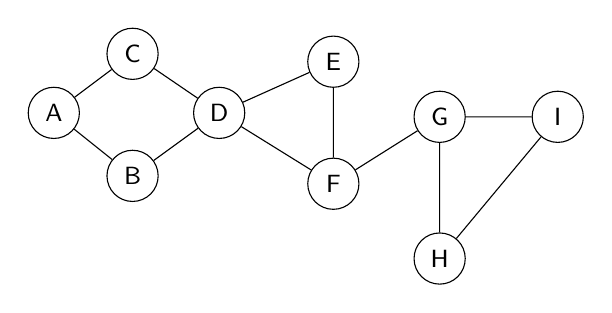
\begin{tikzpicture}[v/.style={circle,draw,minimum size=6.5mm,inner sep=0pt,font=\sffamily\small},x=1cm,y=1cm]
\node[v] (A) at (0,0) {A};
\node[v] (C) at (1.0,0.75) {C};
\node[v] (B) at (1.0,-0.8) {B};
\node[v] (D) at (2.1,0) {D};
\node[v] (E) at (3.55,0.65) {E};
\node[v] (F) at (3.55,-0.9) {F};
\node[v] (G) at (4.9,-0.05) {G};
\node[v] (I) at (6.4,-0.05) {I};
\node[v] (H) at (4.9,-1.85) {H};
\draw (A)--(C) (A)--(B) (C)--(D) (B)--(D) (D)--(E) (D)--(F) (E)--(F) (F)--(G) (G)--(H) (G)--(I) (H)--(I);
\end{tikzpicture}
\end{center}
\begin{enumerate}[label=\Alph*.]
\item (A, C, E, G)
\item (B, F, G, I)
\item (A, B, G)
\item (D, F, G)
\item None of the above
\end{enumerate}
\end{pastexam}

\begin{pastsoln}
答案是 D（D, F, G）。

沿用第 7 題的 DFS 樹（見歷屆試題~\ref{px:ccu-114-csb-07}）：$d$ 依 A, B, \ldots, I 是 $(1, 2, 4, 3, 5, 6, 7, 8, 9)$，$\mathit{low}$ 是
$(1, 1, 1, 1, 3, 3, 7, 7, 7)$。 用資結書定理~23.8、23.9：
\begin{itemize}
\item 根 A 在 DFS 樹裡只有一個子節點 B，不是割點。
\item B：子節點 D 的 $\mathit{low} = 1 < d[B] = 2$，不是。
\item D：子節點 C 的 $\mathit{low} = 1 < 3$；子節點 E 的 $\mathit{low} = 3 \ge d[D] = 3$，是割點。
\item E：子節點 F 的 $\mathit{low} = 3 < 5$，不是。
\item F：子節點 G 的 $\mathit{low} = 7 \ge d[F] = 6$，是割點。
\item G：子節點 H 的 $\mathit{low} = 7 \ge d[G] = 7$，是割點。
\item H：子節點 I 的 $\mathit{low} = 7 < 8$，不是。 C、I 是葉子，不是。
\end{itemize}
割點是 D、F、G，選 D。 直接看圖也對得上：拿掉 D，$\{A, B, C\}$ 和 $\{E, F, \ldots\}$ 分開；拿掉 F，$\{G, H, I\}$ 分開；拿掉 G，
$\{H, I\}$ 和 F 分開。 用第 7 題選項 A 那種走法（C 最後拜訪）算，割點也一樣是 D、F、G。

其他選項：A、B、C 都含有 A、B、C、E 或 I 之一。 A、B、C 在環 A--B--D--C 上，拿掉任一個其他三個仍然相連；E 在三角形 D--E--F 上；
I 在三角形 G--H--I 上。 都不是割點。
\end{pastsoln}
